\documentclass[11pt, a4paper, twocolumn]{article}

\usepackage{fancyhdr} % Required for custom headers
\usepackage{extramarks} % Required for headers and footers
\usepackage{graphicx} % Required to insert images
\usepackage{courier} % Required for the courier font
\usepackage[utf8]{inputenc}
\usepackage{datetime}
\usepackage{amsmath}
\usepackage{amssymb}
\usepackage{arydshln}
\usepackage{mathtools}
\usepackage{pgfplots}
\usepackage{tikz}
\usepackage{multicol}
\usetikzlibrary{arrows,positioning,shapes.geometric}
\usetikzlibrary{plotmarks}
\usepackage[hang,small,bf]{caption}
\usepackage{float}
\usepackage{subcaption}
\usepackage{listings}
\usepackage{hyperref}
\usepackage{epstopdf}
\usepackage[left=1.75cm, right=1.75cm, bottom=3cm, top = 3cm]{geometry}
\usepackage{blindtext}
\usepackage{algorithm}				%För pseudokoder
\usepackage{algpseudocode}			%För pseudokoder
%\usepackage{transparent}
\usepackage{enumitem}
%%\usepackage[table]{xcolor}% http://ctan.org/pkg/xcolor

\newlength\figureheight
\newlength\figurewidth
\newlength\spacing

%%%%%%%%%%%%%%%%%%%%%%% FOR DRAFT %%%%%%%%%%%%%%%%%%%%%%%%%%
\newcommand{\printdraft}{0} % If we want to print draft
%%% USAGE IN TEXT:
% 	\ifnum\printdraft>0
% 		OUR DRAFT TEXT GOES HERE
% 	\else
%   \begin{center}
%   	\textbf{--- DRAFT PARTS ---}
%   \end{center}
%   \fi
%%%%%%%%%%%%%%%%%%%%%%% END DRAFT %%%%%%%%%%%%%%%%%%%%%%%%%%
\linespread{1.0} % Line spacing

% Set up the header and footer
\pagestyle{fancy}
%\lhead{J. Sahlström, A. Lindström \& J. Dürebrandt\\ \today} % Top left header
%\rhead{Project in Modelling Complex Systems} % Right center head
\lhead{\leftmark}
\rhead{\rightmark}
\chead{\firstxmark} % Center right header
\lfoot{\lastxmark} % Bottom left footer
\cfoot{\thepage} % Bottom center footer
%\rfoot{Page\ \thepage\ \protect\pageref{LastPage}} % Bottom right footer
\renewcommand\headrulewidth{0.4pt} % Size of the header rule
\renewcommand\footrulewidth{0.4pt} % Size of the footer rule
\newcommand\bigforall{\mbox{\LARGE $\mathsurround0pt\forall$}}  % Large for all symbol
\setlength{\columnsep}{30pt}
\setlength\parindent{0pt} % Removes all indentation from paragraphs

%----------------------------------------------------------------------------------------
%   TITLE PAGE
%----------------------------------------------------------------------------------------

\title{
%\includegraphics[width=0.3\textwidth]{../img/uu-logo.pdf}\\
Decision-making in Traveling Animal Groups \\ \Large \emph{Project in Modelling Complex Systems}}
\author{
Jakob Sahlström \\ \scriptsize{jasa5691@student.uu.se} 
\and
Anders Lindström \\ \scriptsize{anli6945@student.uu.se} 
\and
Jesper Dürebrandt \\ \scriptsize{jedu6357@student.uu.se}
}
\date{Uppsala University\\\ \\\today} % Insert date here if you want it to appear below your name

%----------------------------------------------------------------------------------------

\usepackage{eso-pic}
\newcommand\BackgroundPic{%
\put(0,0){%
\parbox[b][1.66\paperheight]{\paperwidth}{%
\vfill
\centering

\includegraphics[width=.8\paperwidth,height=.8\paperheight,trim=0 40 0 0, clip,%
keepaspectratio]{img/uu-logo3.pdf}%
%{\transparent{0.20}\includegraphics[width=.8\paperwidth,height=.8\paperheight,trim=0 40 0 0, clip,%
%keepaspectratio]{img/uu-logo.pdf}}%
\vfill
}}}

\begin{document}
\AddToShipoutPicture*{\BackgroundPic}
\twocolumn[
\begin{@twocolumnfalse}
\maketitle
% \begin{abstract}
% \input{sections/abstract.tex}
% \end{abstract}
\end{@twocolumnfalse}
]
%\maketitle
%\thispagestyle{empty}
%\newpage
\setcounter{page}{1}
%\newpage
% \tableofcontents
% \newpage

\section{Introduction}
The direction of movement in animal groups depends on social interaction and the knowledge of certain group members. 
If some group members know where to find food, they will hopefully lead the rest of the group there. 
But how many informed members are required as a function of group size in order to lead the rest if they don't communicate? 
This project implements a model that simulates the movement of a group where the members are oblivious of which members, if any, know where to go.

\section{Model Description}
% A group contains $N$ individuals, where each individual $i$ has a position vector $\boldsymbol{c}_i(t)$, direction as a scalar $d_i(t)$ defined as counter-clockwise angle from the positive x-axis, and speed $s$. 
% The individuals avoid collisions with their neighbors by turning away from individuals $j$ within distance $\alpha$ according to
% \begin{equation}
% d_i (t+\Delta t) = \arg \left(- \sum_{j \neq i} \frac{\boldsymbol{c}_j (t) - \boldsymbol{c}_i (t)}{|\boldsymbol{c}_j (t) - \boldsymbol{c}_i (t) |}\right),
% \label{eq:repulsion}
% \end{equation}
%  where $\arg$ refer to angle to the positive x-axis of of the resulting vector inside the parenthesis and $d_i(t)$ is the desired direction of motion. 
%  If there are no neighbors within distance $\alpha$, the individuals will move towards individuals $j$ within distance $\rho$ according to
% \begin{equation}
% d_p (t) = \arg \left(\sum_{j \neq i} \frac{\boldsymbol{c}_j (t)- \boldsymbol{c}_i (t)}{|\boldsymbol{c}_j (t) - \boldsymbol{c}_i (t)|} \right),
% \label{eq:dp}
% \end{equation}

% \begin{equation}
% d_d (t) = \text{mean}\left( \sum_{j = 1} d_j (t) \right),
% \label{eq:dd}
% \end{equation}

% \begin{equation}
% d_i (t+\Delta t) = \frac{d_p (t) + d_d (t)}{2}.
% \label{eq:attraction}
% \end{equation}
% Here $d_p$ is the direction from individual $i$ to individual $j$, and $d_d$ is the mean value of the directions of the individuals $j$.
% A proportion $p$ of the individuals know in which direction $g$ to go, and their desired direction is given by
% \begin{equation}
% d_i^\prime (t+\Delta t) = d_i (t+\Delta t) + \omega (g - d_i (t+\Delta t)),
% \label{eq:attraction}
% \end{equation}
% where $\omega$ decides the influence of the known direction $g$; $\omega=0$ makes the individual move only by social interaction and the higher the value of $\omega$, the more the individual moves in the known direction.
% \\\\
% A small random angle $\theta$ is added to 





A group contains $N$ individuals, where each individual $i$ has a position vector $\boldsymbol{c}_i(t)$, direction vector $\boldsymbol{v}_i(t)$ and speed $s$. 
The individuals avoid collisions with their neighbors by turning away from individuals $j$ within distance $\alpha$ according to
\begin{equation}
\boldsymbol{d}_i (t+\Delta t) = - \sum_{j \neq i} \frac{\boldsymbol{c}_j (t) - \boldsymbol{c}_i (t)}{|\boldsymbol{c}_j (t) - \boldsymbol{c}_i (t) |},
\label{eq:repulsion}
\end{equation}
where $\boldsymbol{d}_i(t)$ is the desired direction of motion. 
If there are no neighbors within distance $\alpha$, the individuals will move towards individuals $j$ within distance $\rho$ according to
\begin{equation}
\boldsymbol{d}_i (t+\Delta t) = \sum_{j \neq i} \frac{\boldsymbol{c}_j (t)- \boldsymbol{c}_i (t)}{|\boldsymbol{c}_j (t) - \boldsymbol{c}_i (t)|} + \sum_{j = 1} \frac{\boldsymbol{v}_j (t)}{|\boldsymbol{v}_j (t)|}.
\label{eq:attraction}
\end{equation}
The direction $\boldsymbol{d}_i(t)$ is normalized to a unit vector $\hat{\boldsymbol{d}}_i(t)$. 
A proportion $p$ of the individuals know in which direction $\hat{\boldsymbol{g}}$ to go, and their desired direction is given by
\begin{equation}
\boldsymbol{d}_i^\prime (t+\Delta t) = \frac{\hat{\boldsymbol{d}}_i (t+\Delta t) + \omega \hat{\boldsymbol{g}}}{|\hat{\boldsymbol{d}}_i (t+\Delta t) + \omega \hat{\boldsymbol{g}}|},
\label{eq:attraction}
\end{equation}
where $\omega$ decides the influence of the known direction $\hat{\boldsymbol{g}}$; $\omega=0$ makes the individual move only by social interaction and the higher the value of $\omega$, the more the individual moves in the known direction.
\\\\
A small random angle $\theta$ is added to 

\section{Simulation Results}

\newcommand{\myfigwidth}{0.49\linewidth}
\setlength\figurewidth{0.40\linewidth}
\setlength\figureheight{0.40\linewidth}

\begin{figure}[H]
	\centering
	\begin{subfigure}[b]{\myfigwidth}
		\tikzstyle{every node}=[font=\scriptsize]
		% This file was created by matlab2tikz v0.4.7 running on MATLAB 8.2.
% Copyright (c) 2008--2014, Nico Schlmer <nico.schloemer@gmail.com>
% All rights reserved.
% Minimal pgfplots version: 1.3
% 
% The latest updates can be retrieved from
%   http://www.mathworks.com/matlabcentral/fileexchange/22022-matlab2tikz
% where you can also make suggestions and rate matlab2tikz.
% 
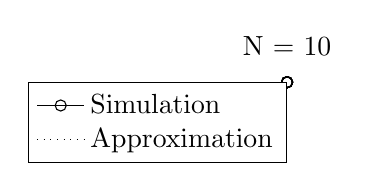
\begin{tikzpicture}

\begin{axis}[%
width=\figurewidth,
height=\figureheight,
unbounded coords=jump,
scale only axis,
xmin=0,
xmax=1,
xlabel={Proportion of informed individuals},
ymin=0,
ymax=10,
ylabel={Elongation},
title={N = 10},
legend style={draw=black,fill=white,legend cell align=left}
]
\addplot [color=black,solid,mark=o,mark options={solid}]
  table[row sep=crcr]{0	0.994143373720641\\
0.1	1.02550613285966\\
0.2	1.20640748601818\\
0.3	1.28533038624398\\
0.4	1.65159642101851\\
0.5	1.8607210442573\\
0.6	1.73468615483567\\
0.7	1.82915697876139\\
0.8	1.74592126576703\\
0.9	1.42801543588063\\
1	1.42268691375327\\
};
\addlegendentry{Simulation};

\addplot [color=black,dotted]
  table[row sep=crcr]{0	-inf\\
0.1	-44.8700576850888\\
0.2	inf\\
0.3	31.8804418757714\\
0.4	14.6568542494924\\
0.5	9.16227766016838\\
0.6	6.52072594216369\\
0.7	4.98975845794461\\
0.8	4\\
0.9	3.31220710410019\\
1	2.80901699437495\\
};
\addlegendentry{Approximation};

\end{axis}
\end{tikzpicture}%
		\caption{Actual distribution in box.}
		\label{fig:elong10}
	\end{subfigure}
	~
	\begin{subfigure}[b]{\myfigwidth}
		\tikzstyle{every node}=[font=\scriptsize]
		% This file was created by matlab2tikz v0.4.7 running on MATLAB 8.2.
% Copyright (c) 2008--2014, Nico Schlmer <nico.schloemer@gmail.com>
% All rights reserved.
% Minimal pgfplots version: 1.3
% 
% The latest updates can be retrieved from
%   http://www.mathworks.com/matlabcentral/fileexchange/22022-matlab2tikz
% where you can also make suggestions and rate matlab2tikz.
% 
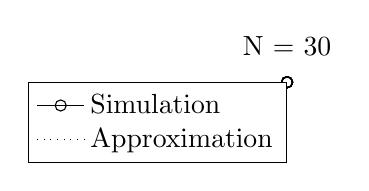
\begin{tikzpicture}

\begin{axis}[%
width=\figurewidth,
height=\figureheight,
unbounded coords=jump,
scale only axis,
xmin=0,
xmax=1,
xlabel={Proportion of informed individuals},
ymin=0,
ymax=10,
ylabel={Elongation},
title={N = 30},
legend style={draw=black,fill=white,legend cell align=left}
]
\addplot [color=black,solid,mark=o,mark options={solid}]
  table[row sep=crcr]{0	1.00301535072817\\
0.1	1.03205098421723\\
0.2	1.29504911983557\\
0.3	3.09125904689578\\
0.4	3.00358256435899\\
0.5	2.78090658125569\\
0.6	2.36526002042314\\
0.7	2.04992392129237\\
0.8	1.78922882325996\\
0.9	1.36911901935186\\
1	1.20710100939255\\
};
\addlegendentry{Simulation};

\addplot [color=black,dotted]
  table[row sep=crcr]{0	-inf\\
0.1	104.54030511288\\
0.2	22.29422863406\\
0.3	11.7202329371918\\
0.4	7.75959179422654\\
0.5	5.72551359424269\\
0.6	4.5\\
0.7	3.68608743668648\\
0.8	3.10874112933697\\
0.9	2.6792584956082\\
1	2.34807023901482\\
};
\addlegendentry{Approximation};

\end{axis}
\end{tikzpicture}%
		\caption{Approximated distribution.}
		\label{fig:elong30}
	\end{subfigure}
	\\
	\begin{subfigure}[b]{\myfigwidth}
		\tikzstyle{every node}=[font=\scriptsize]
		% This file was created by matlab2tikz v0.4.7 running on MATLAB 8.2.
% Copyright (c) 2008--2014, Nico Schlmer <nico.schloemer@gmail.com>
% All rights reserved.
% Minimal pgfplots version: 1.3
% 
% The latest updates can be retrieved from
%   http://www.mathworks.com/matlabcentral/fileexchange/22022-matlab2tikz
% where you can also make suggestions and rate matlab2tikz.
% 
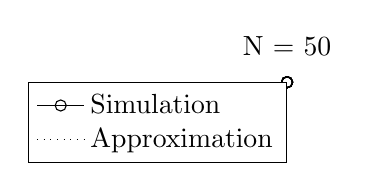
\begin{tikzpicture}

\begin{axis}[%
width=\figurewidth,
height=\figureheight,
unbounded coords=jump,
scale only axis,
xmin=0,
xmax=1,
xlabel={Proportion of informed individuals, p},
ymin=0,
ymax=10,
ylabel={Elongation},
title={N = 50},
legend style={draw=black,fill=white,legend cell align=left}
]
\addplot [color=black,solid,mark=o,mark options={solid}]
  table[row sep=crcr]{0	1.02034692352163\\
0.1	1.09289035466909\\
0.2	1.20577695632396\\
0.3	3.95680389947455\\
0.4	3.72778674107091\\
0.5	3.55498346370831\\
0.6	2.96997739867156\\
0.7	2.47071768260361\\
0.8	1.9452728503174\\
0.9	1.67910478982234\\
1	1.50828773014056\\
};
\addlegendentry{Simulation};

\addplot [color=black,dotted]
  table[row sep=crcr]{0	-inf\\
0.1	52.6944251810664\\
0.2	17.2811529493745\\
0.3	9.92597012245842\\
0.4	6.84990118229706\\
0.5	5.18318275806941\\
0.6	4.1454972243679\\
0.7	3.44054460367719\\
0.8	2.93201073328944\\
0.9	2.54872135086707\\
1	2.25\\
};
\addlegendentry{Approximation};

\end{axis}
\end{tikzpicture}%
		\caption{Approximated distribution.}
		\label{fig:elong50}
	\end{subfigure}
	~
	\begin{subfigure}[b]{\myfigwidth}
		\tikzstyle{every node}=[font=\scriptsize]
		% This file was created by matlab2tikz v0.4.3.
% Copyright (c) 2008--2013, Nico Schlmer <nico.schloemer@gmail.com>
% All rights reserved.
% 
% The latest updates can be retrieved from
%   http://www.mathworks.com/matlabcentral/fileexchange/22022-matlab2tikz
% where you can also make suggestions and rate matlab2tikz.
% 
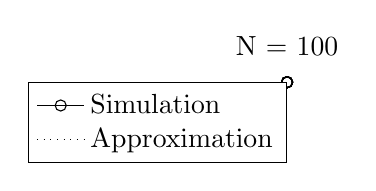
\begin{tikzpicture}

\begin{axis}[%
width=\figurewidth,
height=\figureheight,
unbounded coords=jump,
scale only axis,
xmin=0,
xmax=1,
xlabel={Proportion of informed individuals},
ymin=0,
ymax=10,
ylabel={Elongation},
title={N = 100},
legend style={draw=black,fill=white,legend cell align=left}
]
\addplot [
color=black,
solid,
mark=o,
mark options={solid}
]
table[row sep=crcr]{
0 0.99547989327611\\
0.1 1.08654334799565\\
0.2 6.53913064364081\\
0.3 8.169192332035\\
0.4 5.22493239088512\\
0.5 5.08763539124752\\
0.6 4.30158665907168\\
0.7 3.48136690684954\\
0.8 2.87218165405375\\
0.9 2.27742230081664\\
1 1.79634021711085\\
};
\addlegendentry{Simulation};

\addplot [
color=black,
dotted
]
table[row sep=crcr]{
0 inf\\
0.1 20\\
0.2 10\\
0.3 6.66666666666667\\
0.4 5\\
0.5 4\\
0.6 3.33333333333333\\
0.7 2.85714285714286\\
0.8 2.5\\
0.9 2.22222222222222\\
1 2\\
};
\addlegendentry{Approximation};

\end{axis}
\end{tikzpicture}%
		\caption{Approximated distribution.}
		\label{fig:elong100}
	\end{subfigure}
	\caption{Approximation of particle distribution inside bounding box.}
	\label{fig:elong}
\end{figure}


\section{Analytical Results}
\input{sections/ana_result.tex}

\section{Conclusions}%
\label{sec:conc_future}
The simulations show that the group eventually moves in the correct direction even if only a small proportion of the group is informed. 
In fact, the larger the group, the smaller the proportion of informed individuals is required in order to lead the group in the correct direction as shown in Figure \ref{fig:accuracy}.
\\\\
Furthermore, it can be observed that the portion of individuals to be informed has to overcome a kind of threshold before the elongation goes higher than about one. 
When the portion of informed individuals are low, the elongation is one, but after this threshold there are enough informed individuals to direct the whole group to towards the goal. 
The elongation is at first high, due to the fact that we have the informed individuals in front and the others following them. 
With a larger portion of informed individuals, the driving individuals gets larger, and thereby there will be a wider group, bringing the elongation back towards one.
\\\\
We can observe in Figure \ref{fig:elong10}-\ref{fig:elong100} that the simulation looks like converging to the analytical model, $\frac{1}{p\omega}$.
\\\\
Our results follow the general results of \cite{theArticle} but because of the significant amount of time required for one simulation we did not manage to achieve the same resolution as Couzin et al.

% \bibliographystyle{plain}
% \bibliography{bibliography}
% \nocite{*}

% \begin{thebibliography}{99}
% 	\bibitem{nb_thoery}\href{http://www.aaai.org/Papers/FLAIRS/2004/Flairs04-097.pdf}{Harry Zhang, The Optimality of Naive Bayes, AA, 2004}
% 	\bibitem{nb_comparison}\href{http://citeseerx.ist.psu.edu/viewdoc/download?doi=10.1.1.65.9324&rep=rep1&type=pdf}{McCallum and K. Nigam. “A Comparison of Event Models for Naive Bayes Text Classification” }
% \end{thebibliography}

\end{document}
